\documentclass{article}

\usepackage{tikz}

\usepackage[utf8]{inputenc}


\usetikzlibrary{arrows,decorations.pathmorphing, decorations.pathreplacing,
  backgrounds,fit,positioning,shapes.symbols,chains}
\usepackage[graphics,tightpage,active]{preview}
\PreviewEnvironment{tikzpicture}

 
\begin{document}
\sffamily
%%
%% draw a 4x4 grid such that bottom-left corner is at (#1,0) and fill the frame at (#2,#3) with color #4
%%
\newcommand{\GridOneByte}[4]{
  \begin{tikzpicture}[scale=0.5]
    \foreach \x in {0,...,3} {
      \foreach \y in {0,...,3} {
        \draw (\x+#1,\y) rectangle (\x+#1+1,\y+1); 
      }
    }
    \draw[fill=#4] (#1+#2,#3) rectangle (#1+#2+1,#3+1);
  \end{tikzpicture}
}
%%
%% draw a 4x4 grid such that bottom-left corner is at (#1,0) and fill the column #2 with color #3
%%
\newcommand{\GridOneColumn}[3]{
  \begin{tikzpicture}[scale=0.5]
    \foreach \x in {0,...,3} {
      \foreach \y in {0,...,3} {
        \draw (\x+#1,\y) rectangle (\x+#1+1,\y+1); 
      }
      \draw[fill=#3] (#1+#2,\x) rectangle (#1+#2+1,\x+1);
    }
  \end{tikzpicture}
}

%%
%% draw a 4x4 grid such that bottom-left corner is at (#1,0) and fill some frames with color #4
%%
\newcommand{\GridShiftRows}[2]{
  \begin{tikzpicture}[scale=0.5]
    \foreach \x in {0,...,3} {
      \foreach \y in {0,...,3} {
        \draw (\x+#1,\y) rectangle (\x+#1+1,\y+1); 
      }
    }
    \draw[fill=#2] (#1,3) rectangle (#1+1,4);
    \draw[fill=#2] (#1+1,0) rectangle (#1+2,1);
    \draw[fill=#2] (#1+2,1) rectangle (#1+3,2);
    \draw[fill=#2] (#1+3,2) rectangle (#1+4,3);
  \end{tikzpicture}
}


\definecolor{bleu}{RGB}{0,81,158} % OTBlue
\definecolor{rouge}{RGB}{226,0,43}     % OTRed


\begin{tikzpicture}[->, >=latex, node distance=4.5cm, text width=2cm, text centered, font=\sffamily\bfseries]
\node (A) {\GridOneByte{0}{0}{3}{bleu!80}};
\node (B) [right of=A]{\GridOneColumn{0}{0}{bleu!80}};
\draw (A) -- (B) node [midway, above, sloped] {MixColumns};

\begin{scope}[node distance=2cm, text width=0.5cm]
  \node (key) [right of=B] {\LARGE$\oplus$};
\end{scope}
\begin{scope}[node distance=1.5cm]
  \node (key picture) [above of=key] {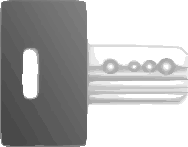
\includegraphics[width=1cm]{key2.pdf}};
\end{scope}
\begin{scope}[node distance=3.5cm]
  \node (C) [right of=key] {\GridOneColumn{6}{0}{rouge!80}};
\end{scope}


\draw (key picture) -- (key);
\draw (B) -- (key);

\draw (key) -- (C) node [midway, above, sloped] {SubBytes};

\node (D) [right of=C] {\GridShiftRows{12}{rouge!80}};
\draw (C) -- (D) node [midway, above, sloped] {ShiftRows};





% \node (D) [right of=A] {\GridOneColumn{6}{0}{yellow!50}};
% \node (C) [right of=B] {\GridOneByte{12}{1}{2}{blue!80}};


\end{tikzpicture}
\end{document}